\NextFile{basic-usage.html}

\chapter{Basic Usage} \label{chap:basic_usage}

This chapter is intended to provide new printer owners with basic information pertaining to the initial setup of their printer in order to help them familiarize themselves with their printer and accomplish a first print.  The information here is a supplement to the documentation which accompanied your printer --- the information specific to your make and model of 3D printer.

\NextFile{basic-usage-leveling.html}

\section{Leveling the Build Plate} \label{sec:leveling}
\index{Tramming|see {Leveling}}
\index{Leveling|(}

The first step towards ensuring the success of a 3D print is making certain that the build plate --- the surface atop which the 3D print is printed --- is well ``trammed'' to the extruder nozzle.  Despite the fact that this process is commonly referred to as ``leveling'', you should not \emph{use} a level as you are not leveling the plate to the horizon.  In actuality, you are making sure that the top surface of the build plate is parallel to the plane the extruder nozzle travels in.  While machinists call this ``tramming'', in the world of 3D printing this is called ``leveling''.

\begin{bclogo}[logo=\bcattention, noborder=true, couleurBarre=red]{Important}
If your printer features auto-leveling or assisted-leveling, then consult the directions for your printer to check whether or not you should manually level the build plate.  It is strongly advised that you follow your printer's specific directions for initial setup.  Often, printers with these features arrive already leveled and merely require some printer specific ``first run'' checks.
\end{bclogo}

Before beginning:

\begin{enumerate}
\item Check your printer's documentation to determine where the build plate's leveling adjustments are.  Most printers have either three or four leveling adjustments.
\item Once the leveling adjustments are identified, determine how to adjust them to raise and lower the plate.  A common form of adjustment is a threaded stud with thumbnut.  If you are looking down towards the top of the plate, you then turn the thumbnut clockwise to raise the plate and counterclockwise to lower the plate.
\item Find a sheet of paper to use as a ``feeler gauge''.  You will use this to set a consistently small gap between the tip of the extruder nozzle and the top of the build plate.  \Glspl{slicer} typically assume this gap to be about 0.1~mm --- approximately the thickness of a sheet of paper.  If you have actual automotive or machinist's feeler gauges, then use such a gauge instead.
\item If your build plate requires a surface treatment (such as tape) which is not already applied, then apply it now before leveling.  Some build plates, such as those provided with ZYYX printers, do not require any treatment.  Most build plates have an aluminum or glass surface that requires a treatment of Kapton (polyimide) tape for ABS or blue ``painter's'' tape for PLA.  Often, these plates come shipped with tape already applied.  Like your filament, the tape is a ``consumable'' and will need to be replaced in time.  Note that if your plate requires a treatment but is shipped without one, then you need to decide with what type of plastic you will be printing.  If you will not be using ABS or PLA, consult the directions that came with your printer.
\end{enumerate}

To level your build plate for the first time, the procedure is as follows.  Again, note that you should consult the documentation that accompanied your printer to check for printer-specific instructions, as the following instructions are generic by necessity:

\begin{enumerate}
\item Adjust the leveling points in order to lower your build plate relative to its support mechanism (e.g., support arms).  This does not mean you should lower the entire assembly down the Z rods.  Rather, compress the springs on which the build plate rides and tighten the thumbnuts, thereby lowering the plate itself in relation to the arms and other structures supporting it.  This ensures that there is a significant gap between the nozzle and the build plate's surface in order to reduce the risk of damaging either.
\item Remove any debris from the tips of the extruder nozzles.  If there is a small bead of plastic, it can be broken off with small tweezers.
\item Turn on the printer.
\item From the main menu (Section \ref{sec:Main}) of your LCD display, select the ``Utilities'' menu (Section \ref{sec:utilities}) by pressing the down key twice and then pressing the center key.  The keypad and the LCD screen are normally located close to each other somewhere on the front of the printer.
\item Within the Utilities menu, press the down key to scroll downwards until you have selected the ``Home Axes'' item (Section~\ref{sec:home-axes}).  Press the center key to choose the item.
\item Having selected ``Home Axes'', the printer will move the extruders to the back, right corner.  Then the printer will raise the build platform twice, slowly the second time.
\item Once this homing operation is completed, manually slide the extruder assembly over the build surface, ensuring that it does not touch the top of the build surface anywhere.  If it does, then continue to lower the build surface using the leveling adjustments.  If the build surface cannot be lowered further and the extruder is still hitting it, either the Z endstop\footnote{The Z endstop is typically a limit switch which, when triggered, stops further upward motion of the build plate.  Consult your printer manual for information on the location and adjustment of this endstop.} may need to be lowered or a shim should be installed, after which Steps~5, 6, and 7 should be repeated.
\item Before beginning leveling, you need to heat up the build plate if you will be printing with it heated.  As some heated build surfaces expand a small amount or may even ``crown'' upwards in the middle a little when heated, the plate must be leveled in its operational configuration.  From the keypad press the left key to return to the main menu, then scroll up using the up key and select the Preheat item by pressing the center key, Section~\ref{sec:preheat}.  Make sure you are not heating the extruders by scrolling to their lines and pressing the center key to toggle the value to ``OFF''.  Likewise, ensure that the heating platform reads ``ON'' before scrolling up to the first line and pressing the center key to begin preheating.  A monitor screen will appear, similar to the one shown in Figure \ref{fig:tempform}.  Wait until the platform reaches its target temperature, which is usually 100\textdegree\,C for ABS or 50\textdegree\,C for PLA; the temperatures are displayed in the form current temperature/target temperature in degrees Celsius.  Once the platform is fully heated, press the left key to return to the main menu.

\begin{figure}[!htbp]
  \centering
    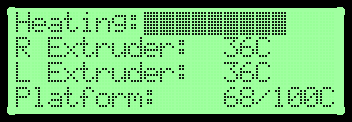
\includegraphics[]{preheat-monitor-01}
    \caption{Monitor Screen}
  \label{fig:tempform}
\end{figure}

\item From the Utilities menu, scroll down until you reach ``Level Build Plate'', then select it using the center key, Section~\ref{sec:levelbp}.
\item The printer will now home its axes as before, then move the nozzle to the approximate center of the build plate.  Directions will appear on the LCD screen; press the center key to advance from screen to screen.  The final screen will be the one depicted in Figure \ref{fig:level-01}.

\begin{figure}[!htbp]
  \centering
    
\includegraphics[]{level-01}
    \caption{Leveling}
  \label{fig:level-01}
\end{figure}

\item To level the build plate, manually move the extruder so that the nozzle is roughly over one of the adjustment points.  Take care to avoid dragging the nozzle across the build surface, as that may cause damage.  Then, adjust the point so that there is only a small gap between the tip of the nozzle and the top of the build surface.  Place the piece of paper between the two as you adjust.  You want to be able to slide the paper back and forth, but with some friction.
\item After you are satisfied that this point is adjusted, move the extruder to the next point to repeat the process.  Do not press the center key yet.
\item Once you have finished adjusting all the points, recheck them.  You may also wish to check the center of the build plate.  The plate may crown a little when heated and the long X rods supporting the extruder can sag a tiny amount.  As such, you may find the gap to be too small at the center.  If so, you may need to fiddle with the adjustment points until a more uniform gap across the plate is achieved.\footnote{For small, centered prints, having a 0.1~mm gap near the plate's center is critical and a slightly larger gap at the edges can be tolerated.  However, when doing large prints, it may be necessary to print with a \gls{raft} or to obtain a flatter build surface.  See your slicer's documentation for information on generating rafts.}  Note that turning all thumbnuts by an equal amount will raise or lower the entire plate evenly.
\item If you have finished checking and rechecking all your test points, and you are satisfied that the plate is level, then press the center key.  Now that you have completed leveling, you are ready to load filament.
\end{enumerate}

\begin{bclogo}[logo=\bcinfo, noborder=true, couleurBarre=yellow]{Note}
In general, you do not need to level your build plate before every print.  As you continue to use your printer, the frequency with which you need to level your plate will diminish.  However, in the first week or so you may need to level it every few prints.  This is in part due to your lack of experience, but may also
be the result of your printer settling in.
\end{bclogo}
\index{Leveling|)}

\NextFile{basic-usage-filament-loading.html}

\section{Loading Filament}
\index{Filament!Loading|(}

Before starting your first print, you must first load filament into each extruder you will be using.  However, even if your printer has two extruders, it is strongly recommended that you start with a simple print which uses only a single extruder --- preferably the right extruder.  As such, you should not load filament into the second extruder until you actually need to use it.

Most 3D printers come with a spool or two of filament, which is generally either ABS or PLA plastic.  While the loading directions are the same regardless, you should load a filament compatible with the treatment applied to the surface of your build plate (e.g., ABS for Kapton tape on the build surface; PLA for painter's tape on the build surface).

From the documentation for your printer, you will need to determine:

\begin{enumerate}
\item The proper filament spool mounting technique.  Many printers come with a rear-mounted filament spool.
\item The spool orientation and filament feed path.  It is important to set this up properly so as to prevent filament tangles and other feed-related problems.
\item The mechanical steps to load filament into your extruder's feed mechanism, as this varies between printers.
\end{enumerate}

Once you have determined the above information, you are ready to load filament into your extruder --- the righthand extruder if you have two:

\begin{enumerate}
\item With a pair of scissors, neatly trim the end of the filament.  Mount the filament spool in its correct orientation and feed the filament through any guide tubes along its feed path.  Do not yet attempt to load the filament into the extruder itself.
\item Turn on your printer.  Then, from the front LCD panel navigate with the down key to the ``Utilities'' item, Section \ref{sec:utilities}.  Press the center key to select it.
\item Within the Utilities menu, navigate to the line reading ``Filament Loading'' (Section~\ref{sec:filload}).  Again, press the center key to select this.
\item If your printer arrived with a short length of filament already loaded into the extruder, then you will want to unload it first:
\begin{enumerate}
\item Select ``Unload Filament'' and the printer will heat up the extruder to the temperature set in Preheat Settings under the Utilities menu, Section~\ref{sec:preheatset}.  By default, this is 230\textdegree\,C.  If you have two extruders, select this for the right extruder.
\item Once heated up, the printer will then begin to unload the filament.  After a few moments you should be able to manually pull the segment out.  This should \emph{not} require much force.
\item You may press the center key to stop the unloading process.
\end{enumerate}
\item Now select ``Load Filament''.  If you have two extruders, select loading
for the right extruder.
\item The printer will now begin to heat up the extruder to the temperature set in Preheat Settings under the Utilities menu.
\item Once the extruder has reached temperature, the front LCD panel will generate a screen telling you to begin loading the filament into the extruder.  The feed motor for the extruder will begin turning to allow you to load the filament.  Following the necessary procedure for your printer, load the filament into the extruder and allow it to feed the filament.
\item After a few moments, a hot plastic thread will begin to emerge from the extruder's nozzle.  If it is not initially the color of the filament you loaded, note that the factory may have tested the printer using a different color filament.  Allow the filament to extrude for at least 30 seconds before pressing the center key to stop the process.  Press the left key once to return to the Utilities menu; press the left key a second time to return to the top-level menu.
\end{enumerate}

\begin{bclogo}[logo=\bcinfo, noborder=true, couleurBarre=yellow]{Note}
If the extruded filament tends to curl upwards as it exits the nozzle, then there may be debris clogging the nozzle.  If such is the case, contact your printer manufacturer for assistance.  Also, if the extruded filament bubbles and pops a little, then your filament has absorbed too much moisture and may need to be dried out.  The proper way of drying it depends on the type of filament; contact your filament vendor for guidance.
\end{bclogo}

\index{Filament!Loading|)}

\NextFile{basic-usage-starting-a-print.html}

\section{Starting a Print}

\begin{bclogo}[logo=\bcattention, noborder=true, couleurBarre=red]{Important}
Do not leave your printer operating unattended!  Unless your printer manufacturer expressly states that your printer supports unattended operation, you must not allow it to operate unsupervised.  There have been cases of 3D printers failing and burning themselves down.  Unattended printing carries significant risk to life and property.  Be Safe!
\end{bclogo}

Most printers ship with an \gls{SD card} containing sample prints.  For your first print choose a sample that only requires the use of a single extruder.  If such a card was not supplied, then you will need to obtain a model and prepare it for printing with a \gls{slicer}.  Explaining this procedure is outside the scope of this document due to the numerous variables arising from printer, slicer, etc.\ variations.

Insert the SD card into the printer's SD card slot, and then turn on the printer.  From the main menu of the LCD screen select the ``Print From SD'' option, select the file you wish to print --- note that, if there are more than four files on the SD card, you may have to scroll down --- and then the print will begin.\footnote{For more details on navigating the ``Print From SD'' menu, finding hidden files, and making your files accessible see Section \ref{sec:sdmenu}.}  The print monitor screen will be generated; for more details see Section \ref{sec:printmon}.

\NextFile{basic-usage-tips.html}

\section{Tips}

Now that you have completed a print or two, here is further advice to help ensure your continued success.  Moving forward, keep in mind
that the most common problem people experience is getting the first layer
of their print to adhere properly to the build plate.  Here are some tips
which may prove helpful:

\begin{enumerate}
\item Properly leveling your build plate is critical to successful
printing.  Also, be consistent: use the same sort of paper each time or a
0.1~mm feeler gauge.  \emph{Do not eyeball the gap.}
\item Start with 0.30~mm layer height prints.  The lower the layer height, the
more important it is to have properly leveled the build plate as well as having a very flat
(non warped) build plate.  As you continue to print, you will get better
at leveling the plate, at which point you can try your hand at 0.20 and even 0.15 or
0.10~mm layer heights.  However, stick with 0.30~mm prints until you are experienced and reasonably skilled.
\item Use the proper build surface treatment.  Some printers such as MBot3D
and ZYYX come with a special build surface that requires no tape. Many other
printers, however, come with just an aluminum or glass plate.  For those
surfaces you need to add tape --- and not just any tape.  Use Kapton tape
(polyimide) for ABS prints and blue ``painter's'' tape for PLA.  Occasionally
wipe down the Kapton with acetone or the painter's tape with alcohol.  ABS
also requires a heated build plate to adhere well.
\item The ideal extrusion temperature for each filament type may differ.  While you should begin with the printer manufacturer's recommendations, you may wish to experiment some with higher or lower temperatures in order to find the optimum temperatures.
\end{enumerate}

\ifdefined\luluflag
\pagebreak[4]
\fi

\NextFile{basic-usage-next-steps.html}

\section{Next Steps}

Enjoy your printer!

Early on, you should perform basic printer calibrations.  For guidance, see Chapter~\ref{chap:tuning}.

Visit \myhref{http://thingiverse.com/}{Thingiverse} for an astounding
collection of printable models.  When you find a model you want to
print, check to see if there is advice for slicer settings.  Such information
is often found in the description or instruction sections of the
Thingiverse page for the model.  Gravitate towards models which have
actual pictures of the printed item as some models posted will not print easily --- or at all.  Seeing a photo of an actual print provides extra assurance that the model is sound.

After you have used your printer and slicer for a few weeks, branch
out and look at some other slicers.  Each slicer has
its own strengths and weaknesses.  Many of the slicers are under
active development, receiving new improvements regularly.  Keep in
mind, however, that MakerBot-style printers consume a format called
X3G (Section~\ref{sec:s3g-x3g}).  The gcode from your slicer is
converted to that format for you.  As of this writing, the slicers
which automatically perform this conversion for you are MakerBot
Desktop, MakerBot MakerWare, ReplicatorG -- Sailfish, and
Simplify3D.\footnote{Active development of Skeinforge, the slicer within
ReplicatorG, ceased in April 2012.}
While you can use other slicers such as Cura, KISSlicer, and slic3r,
you will need to use a tool to convert their gcode to X3G.  The
two common approaches are to either import the gcode into a slicer which
handles X3G or to use the \gls{GPX} tool to do the conversion.  GPX may be
found at Thingiverse as
\myhref{http://www.thingiverse.com/thing:81425}{Thing \#81425}.\index{GPX}

Finally, search out any user groups for your brand of printer.  Some
manufacturers run or link to online forums from their own web pages.
Other printer groups may be found at sites such as
\myhref{http://groups.google.com}{groups.google.com}.
